\documentclass[10pt,winfonts,fancyhdr,hyperref,UTF8]{ctexrep}
\usepackage{indentfirst} 
\usepackage{fontspec}
\usepackage{titlesec}
\usepackage{xeCJK}
\usepackage{graphicx}
\usepackage{ifthen}
\usepackage{color,fancyvrb}
\usepackage{listings}
\usepackage{syntonly}
\usepackage{makeidx}
\usepackage[hidelinks, colorlinks=true]{hyperref}
\usepackage{algorithm}
\usepackage{algpseudocode}
\usepackage{amssymb}
\usepackage{multirow}
\usepackage{ulem}
\usepackage{diagbox}
\makeatletter
%LeetCode Setting
\usepackage[centering,paperwidth=180mm,paperheight=230mm,%
body={390pt,530pt},marginparsep=10pt,marginpar=50pt]{geometry}
\usepackage{color}
\usepackage{enumitem}
\usepackage{fancyvrb}
\usepackage[bottom,perpage,symbol*]{footmisc}
\usepackage{graphicx}
\usepackage[hidelinks]{hyperref}
\usepackage{makeidx}
\usepackage[toc]{multitoc}
\usepackage{pifont}
\usepackage{underscore}
\usepackage{amsmath}

\DefineFNsymbols*{chinese}{{\ding{172}}{\ding{173}}{\ding{174}}{\ding{175}}%
{\ding{176}}{\ding{177}}{\ding{178}}{\ding{179}}{\ding{180}}{\ding{181}}}
\setfnsymbol{chinese}

\hypersetup{bookmarksnumbered=true,bookmarksdepth=2}

\CTEXsetup[number={\thechapter}]{chapter}
\CTEXsetup[format+={\raggedleft}]{chapter}
\CTEXsetup[beforeskip={10pt}]{chapter}
\CTEXsetup[afterskip={30pt}]{chapter}
\def\CTEX@chapter@aftername{\par} % \CTEXsetup[aftername={\par}]{chapter}
\CTEXsetup[format+={\raggedright}]{section}
\CTEXsetup[beforeskip={-3.0ex plus -1ex minus -.2ex}]{section}
\CTEXsetup[afterskip={2.3ex plus .2ex minus 0.2ex}]{section}

\renewcommand \thefigure{\thechapter-\arabic{figure}}
\renewcommand \thetable{\thechapter-\arabic{table}}

\newcommand\figcaption[1]{\def\@captype{figure}\caption{#1}}
\newcommand\tabcaption[1]{\def\@captype{table}\caption{#1}}

\long\def\@caption#1[#2]#3{%
  \addcontentsline{\csname ext@#1\endcsname}{#1}%
    {\protect\numberline{\csname fnum@#1\endcsname}{ \ignorespaces #2}}% change "the" to "fnum@"
    \normalsize
    \@makecaption{\csname fnum@#1\endcsname}{\ignorespaces #3}}

\long\def\@makecaption#1#2{%
  \vskip\abovecaptionskip
  \sbox\@tempboxa{#1\quad#2}%
  \ifdim \wd\@tempboxa >\hsize
    #1\quad#2\par
  \else
    \global \@minipagefalse
    \hb@xt@\hsize{\hfil\box\@tempboxa\hfil}%
  \fi
  \vskip\belowcaptionskip}

\setlength\abovecaptionskip{0pt}
  
\setmainfont{Times New Roman}
%\setmainfont{Linux Libertine}
%\setmainfont{TeX Gyre Pagella}
\newfontfamily\urlfont{Times New Roman}
%\setmonofont[AutoFakeBold=1.6,AutoFakeSlant=0.17,Mapping=tex-text-tt]{Inconsolata}
\setCJKfamilyfont{zhyou}{YouYuan}

\newcommand{\fn}[1]{\texttt{#1}}
\newcommand{\sfn}[1]{\texttt{\small #1}}
\newcommand{\kw}[1]{\textsf{#1}}
\newcommand{\myurl}[1]{{\urlfont #1}}
\newcommand{\mpar}[1]{\marginpar[\hfill\kaishu #1]{\kaishu #1}}
\newcommand{\mn}[1]{\texttt{\bs #1}}
\renewcommand{\today}{\the\year-\the\month-\the\day}
\newcommand\bs{\textbackslash}
\newcommand{\code}[1]{\small{\fontspec{Latin Modern Mono} #1}}

\newcommand\begindot{\begin{itemize}
[itemsep=2pt plus 2pt minus 2pt,%
topsep=3pt plus 2pt minus 2pt,%
parsep=0pt plus 2pt minus 2pt]}
\newcommand\myenddot{\end{itemize}}

\newcommand\beginnum{\begin{enumerate}
[itemsep=2pt plus 2pt minus 2pt,%
topsep=3pt plus 2pt minus 2pt,%
parsep=0pt plus 2pt minus 2pt]}
\newcommand\myendnum{\end{enumerate}}

\DefineVerbatimEnvironment%
  {Code}{Verbatim}
  {fontsize=\small,baselinestretch=0.9,xleftmargin=3mm}

\raggedbottom
%\setlength{\parskip}{1ex plus .5ex minus .5ex}

\def\FV@SetLineWidth{%
  \if@FV@ResetMargins\else
    \advance\leftmargin\@totalleftmargin
  \fi
  \advance\leftmargin\FV@XLeftMargin\relax
  \advance\rightmargin\FV@XRightMargin\relax
  \linewidth\hsize
  %\advance\linewidth-\leftmargin
  %\advance\linewidth-\rightmargin
  \hfuzz\FancyVerbHFuzz\relax}


\def\FV@SingleFrameLine#1{%
%% DG/SR modification end
  \hbox to\z@{%
    %\kern\leftmargin
%% DG/SR modification begin - Jun. 22, 1998
    \ifnum#1=\z@
      \let\FV@Label\FV@LabelBegin
    \else
      \let\FV@Label\FV@LabelEnd
    \fi
    \ifx\FV@Label\relax
%% DG/SR modification end
      \FancyVerbRuleColor{\vrule \@width\linewidth \@height\FV@FrameRule}%
%% DG/SR modification begin - Jun. 22, 1998
    \else
      \ifnum#1=\z@
        \setbox\z@\hbox{\strut\enspace\urlfont\FV@LabelBegin\strut}%
      \else
        \setbox\z@\hbox{\strut\enspace\urlfont\FV@LabelEnd\strut}%
      \fi
      \@tempdimb=\dp\z@
      \advance\@tempdimb -.5\ht\z@
      \@tempdimc=\linewidth
      \advance\@tempdimc -\wd\z@
      %\divide\@tempdimc\tw@
      \ifnum#1=\z@              % Top line
        \ifx\FV@LabelPositionTopLine\relax
          \FancyVerbRuleColor{\vrule \@width\linewidth \@height\FV@FrameRule}%
        \else
          \FV@FrameLineWithLabel
        \fi
      \else                     % Bottom line
        \ifx\FV@LabelPositionBottomLine\relax
          \FancyVerbRuleColor{\vrule \@width\linewidth \@height\FV@FrameRule}%
        \else
          \FV@FrameLineWithLabel
        \fi
      \fi
    \fi
%% DG/SR modification end
    \hss}}


%% DG/SR modification begin - May. 19, 1998
\def\FV@FrameLineWithLabel{%
  \ht\z@\@tempdimb\dp\z@\@tempdimb%
  \FancyVerbRuleColor{%
    \raise 0.5ex\hbox{\vrule \@width\@tempdimc \@height\FV@FrameRule}%
    \raise\@tempdimb\box\z@}}
%% DG/SR modification end


\def\FV@EndListFrame@Lines{%
  \begingroup
    %\vskip 0.5ex
    \baselineskip\z@skip
    \kern\FV@FrameSep\relax
%% DG/SR modification begin - May. 19, 1998
%%    \FV@SingleFrameLine
    \FV@SingleFrameLine{\@ne}%
%% DG/SR modification end
  \endgroup}

\newskip\mytopsep
\setlength{\mytopsep}{4pt plus 2pt minus 3pt}

\def\FV@ListVSpace{%
  \@topsepadd\mytopsep
  \if@noparlist\advance\@topsepadd\partopsep\fi
  \if@inlabel
    \vskip\parskip
  \else
    \if@nobreak
      \vskip\parskip
      \clubpenalty\@M
    \else
      \addpenalty\@beginparpenalty
      \@topsep\@topsepadd
      \advance\@topsep\parskip
      \addvspace\@topsep
    \fi
  \fi
  %\showthe \@topsepadd
  %\showthe \topsep
  %\showthe \partopsep
  %\showthe \parskip
  \global\@nobreakfalse
  \global\@inlabelfalse
  \global\@minipagefalse
  \global\@newlistfalse}

\def\FV@EndList{%
  \FV@ListProcessLastLine
  \FV@EndListFrame
  %\showthe \@topsepadd
  \@endparenv
  \endgroup
  \@endpetrue}

\def\theFancyVerbLine{\sffamily\scriptsize\arabic{FancyVerbLine}}

\DefineVerbatimEnvironment%
  {Codex}{Verbatim}
  {fontsize=\small,baselinestretch=0.9,xleftmargin=3mm,%
  frame=lines,labelposition=all,framesep=5pt}

\DefineVerbatimEnvironment%
  {Code}{Verbatim}
  {fontsize=\small,baselinestretch=0.9,xleftmargin=3mm}

\makeindex

%Other settings:
\lstset{%  
  alsolanguage=Java,  
  language={C++},
  tabsize=4, %  
  frame=shadowbox, %把代码用带有阴影的框圈起来  
  commentstyle=\color{red!50!green!50!blue!50},%浅灰色的注释  
  rulesepcolor=\color{red!20!green!20!blue!20},%代码块边框为淡青色  
  keywordstyle=\color{blue!90}\bfseries, %代码关键字的颜色为蓝色,粗体  
  showstringspaces=false,%不显示代码字符串中间的空格标记  
  stringstyle=\ttfamily, % 代码字符串的特殊格式  
  keepspaces=true, %  
  breakindent=22pt, %  
  numbers=left,%左侧显示行号 往左靠,还可以为right,或none,即不加行号  
  stepnumber=1,%若设置为2,则显示行号为1,3,5,即stepnumber为公差,默认stepnumber=1  
  %numberstyle=\tiny, %行号字体用小号  
  numberstyle={\color[RGB]{0,192,192}\tiny} ,%设置行号的大小,大小有tiny,scriptsize,footnotesize,small,normalsize,large等  
  numbersep=8pt,  %设置行号与代码的距离,默认是5pt  
  basicstyle=\footnotesize, % 这句设置代码的大小  
  showspaces=false, %  
  flexiblecolumns=true, %  
  breaklines=true, %对过长的代码自动换行  
  breakautoindent=true,%  
  breakindent=4em, %  
  aboveskip=1em, %代码块边框  
  tabsize=2,  
  showstringspaces=false, %不显示字符串中的空格  
  backgroundcolor=\color[RGB]{245,245,244},   %代码背景色  
}















\makeatother
%\graphicspath{{images/}}

\usepackage{tikz}
\usetikzlibrary{calc}
\usetikzlibrary{fit}
\usetikzlibrary{positioning}
\usepgflibrary{plotmarks}

\usetikzlibrary{shapes.geometric}

\CustomVerbatimEnvironment{shellcmd}{Verbatim}
{frame=single,rulecolor=\color{blue},framerule=3pt,framesep=1pc,fillcolor=\color{yellow}}

\newcommand{\bookname}{TechNotes}
\renewcommand{\contentsname}{CodingTechniques} 

\title{\sffamily CodingTechniques}
\date{\today}
\setcounter{tocdepth}{1}
\setcounter{chapter}{3}

\begin{document}

%\maketitle
\tableofcontents


%TOADD
%!Mode:: "TeX:UTF-8"
\chapter{编程技巧}

%!Mode:: "TeX:UTF-8"
\section{软件工程开发模型}

\subsection{四大开发模型}
\textbf{瀑布模型(Waterfall Model)}是由W.W.Royce在1970年首次提出的软体开发模型,在瀑布模型中,软件开发被分为需求分析,设计,实现,测试 (确认), 集成,和维护这样的步骤依序进行。Royce提倡重复地使用瀑布模型,以一种迭代的方式。但是,大多数人并不知道这一点,一些人也不相信它能被应用在现实生活中,因为过程很少能够以连续由上而下的方式进行。 经常会需要回到前面的阶段,或改变前一阶段的结果。讽刺的是,在Royce 1970年的那篇文章中他提到:这种模型的目的是作为用来说明这种模式有缺陷,而不适用。事实上,软体开发相关文章中对这个名词的大量引用正是对这个广泛流行的软体开发做法的一种评判。瀑布模型最早强调系统开发应有完整之周期,且必须完整的经历周期之每一开发阶段,并系统化的考量分析与设计的技术、时间与资源之投入等,因此瀑布模型又可以称为‘系统发展生命周期’(System Development Life Cycle, SDLC)。由于该模式强调系统开发过程需有完整的规划、分析、设计、测试及文件等管理与控制,因此能有效的确保系统品质,它已经成为软体业界大多数软件开发的标准。

\textbf{原型模型},即快速应用程式开发 (原名:Rapid Application Development、缩写:RAD)是指一种以最小幅度的规划并迅速地将原形完成的软件发展方法论。采用RAD进行软件开发的规划是和撰写软件本身交错同时进行的。通常能在没有大量预先规划的情况下,让软件更快写完、更容易变更需求。

\textbf{螺旋模型}是一种演化软件开发过程模型,它兼顾了快速原型的迭代的特征以及瀑布模型的系统化与严格监控。螺旋模型最大的特点在于引入了其他模型不具备的风险分析,使软件在无法排除重大风险时有机会停止,以减小损失。同时,在每个迭代阶段构建原型是螺旋模型用以减小风险的途径。螺旋模型更适合大型的昂贵的系统级的软件应用。
\begin{figure}[ht]
	\begin{center}
		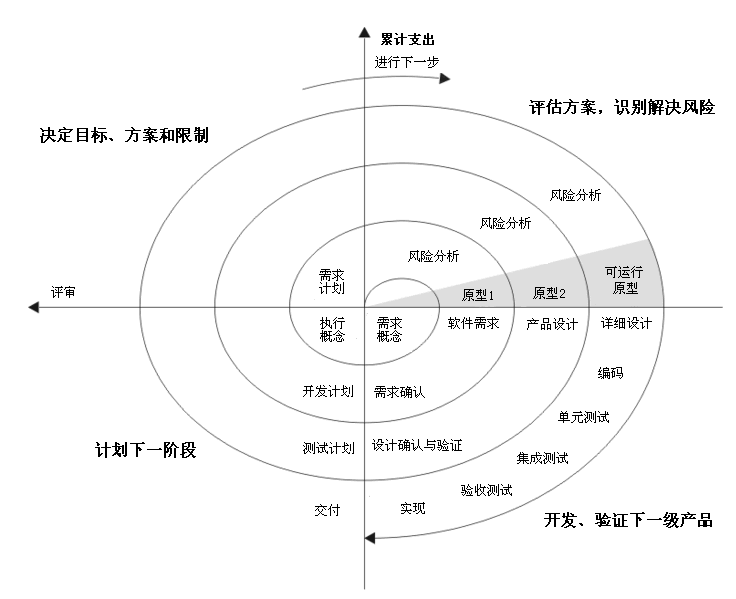
\includegraphics[keepaspectratio,width=0.5\paperwidth]{Pictures/SpiralModelChinese.png}
	\caption{螺旋模型}
	\label{fig:processmemlayout}
	\end{center}
\end{figure}

\textbf{增量模型(incremental build model)}融合了瀑布模型的基本成分(重复应用)和原型实现的迭代特征,该模型采用随着日程时间的进展而交错的线性序列,每一个线性序列产生软件的一个可发布的“增量”。当使用增量模型时,第1个增量往往是核心的产品,即第1个增量实现了基本的需求,但很多补充的特征还没有发布。客户对每一个增量的使用和评估都作为下一个增量发布的新特征和功能,这个过程在每一个增量发布后不断重复,直到产生了最终的完善产品。产品被分解为多个部件,各部件独立设计构建(被称为builds)。每个部件在完成时即时提交给客户,这样就可以利用部分完成的产品,不必等待整个开发期。客户不必一下子接触到一个全新的产品。


\begin{figure}[ht]
	\begin{center}
		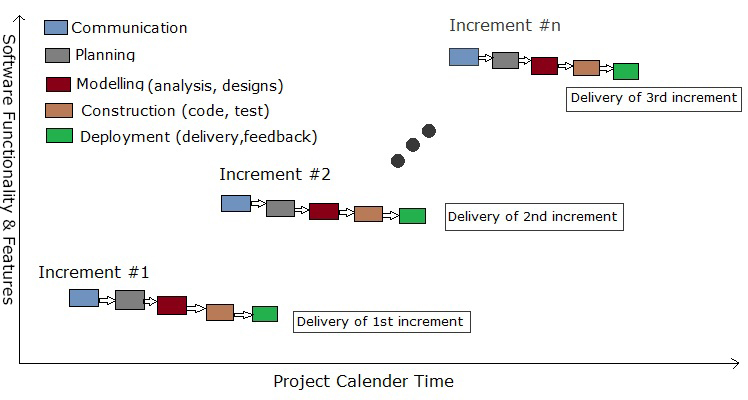
\includegraphics[keepaspectratio,width=0.5\paperwidth]{Pictures/IncrementalModel.jpg}
	\caption{增量模型}
	\label{fig:processmemlayout}
	\end{center}
\end{figure}

\subsection{迭代式开发}
迭代式开发也被称作迭代增量式开发或迭代进化式开发,是一种与传统的瀑布式开发相反的软件开发过程,它弥补了传统开发方式中的一些弱点,具有更高的成功率和生产率。
在迭代式开发方法中,整个开发工作被组织为一系列的短小的、固定长度(如3周)的小项目,被称为一系列的迭代。每一次迭代都包括了需求分析、设计、实现与测试。采用这种方法,开发工作可以在需求被完整地确定之前启动,并在一次迭代中完成系统的一部分功能或业务逻辑的开发工作。再通过客户的反馈来细化需求,并开始新一轮的迭代。

\subsection{敏捷软件开发}
\textbf{敏捷软件开发(Agile software development)},又称敏捷开发,是一种从1990年代开始逐渐引起广泛关注的一些新型软件开发方法,是一种应对快速变化的需求的一种软件开发能力。它们的具体名称、理念、过程、术语都不尽相同,相对于“非敏捷”,更强调程序员团队与业务专家之间的紧密协作、面对面的沟通(认为比书面的文档更有效)、频繁交付新的软件版本、紧凑而自我组织型的团队、能够很好地适应需求变化的代码编写和团队组织方法,也更注重软件开发中人的作用。

敏捷方法有时候被误认为是无计划性和纪律性的方法,实际上更确切的说法是敏捷方法强调适应性而非预见性。
适应性的方法集中在快速适应现实的变化。当项目的需求起了变化,团队应该迅速适应。这个团队可能很难确切描述未来将会如何变化。
相比迭代式开发两者都强调在较短的开发周期提交软件,敏捷方法的周期可能更短,并且更加强调队伍中的高度协作。

通常可以在以下方面衡量敏捷方法的适用性:从产品角度看,敏捷方法适用于需求萌动并且快速改变的情况,如系统有比较高的关键性、可靠性、安全性方面的要求,则可能不完全适合;从组织结构的角度看,组织结构的文化、人员、沟通则决定了敏捷方法是否适用。最重要的因素恐怕是项目的规模。规模增长,面对面的沟通就愈加困难,因此敏捷方法更适用于较小的队伍,40、30、20、10人或者更少。大规模的敏捷软件开发尚处于积极研究的领域。

\subsection{极限编程}
极限编程(Extreme programming,缩写为XP),是一种软件工程方法学,是敏捷软件开发中最富有成效的几种方法学之一。如同其他敏捷方法学,极限编程和传统方法学的本质不同在于它更强调可适应性而不是可预测性。极限编程的支持者认为软件需求的不断变化是很自然的现象,是软件项目开发中不可避免的、也是应该欣然接受的现象;他们相信,和传统的在项目起始阶段定义好所有需求再费尽心思的控制变化的方法相比,有能力在项目周期的任何阶段去适应变化,将是更加现实更加有效的方法。

极限编程为管理人员和开发人员开出了一剂指导日常实践的良方;这个实践意味着接受并鼓励某些特别的有价值的方法。支持者相信,这些在传统的软件工程中看来是“极端的”实践,将会使开发过程比传统方法更加好的响应用户需求,因此更加敏捷,更好的构建出高质量软件。

\subsection{Rational统一过程}
Rational统一过程(RUP)是Rational软件公司(现在Rational公司被IBM并购)创造的软件工程方法。RUP描述了如何有效地利用商业的可靠的方法开发和部署软件,是一种重量级过程(也被称作厚方法学),因此特别适用于大型软件团队开发大型项目。

在软件工程领域,与RUP齐名的软件方法还有:
\begin{itemize}
\item 净室软件工程(重量级)、CMMI(重量级)
\item 极限编程(extreme programming)和其他敏捷软件开发(agile methodology)方法学(轻量级)
\end{itemize}

\subsection{Scrum}

Scrum是一种迭代式增量软件开发过程,通常用于敏捷软件开发。Scrum在英语里是橄榄球运动中争球的意思。
虽然Scrum是为管理软件开发项目而开发的,它同样可以用于运行软件维护团队,或者作为计划管理方法。Scrum之间的合作称为“Scrum of Scrums”。

Scrum是一个包括了一系列实践和预定义角色的过程骨架。Scrum中的主要角色包括:
\begin{enumerate}
\item 'Scrum Master' 是Scrum教练和团队带头人,确保团队合理的运作Scrum,并帮助团队移除实施中的障碍;
\item 产品负责人(Product Owner),确定产品的方向和愿景,定义产品发布的内容、优先级及交付时间,为产品投资报酬率(ROI)负责;
\item 开发团队(Team),一个跨职能的小团队,人数3-9人,团队拥有交付可用软件需要的各种技能。
\end{enumerate}

在每一次冲刺(a sprint or iteration, 一个15到30天的周期,其长度由开发团队决定)当中,开发团队创建可用的(可以随时推出)软件的一个增量。每一个冲刺所要实现的功能来自产品订单(product backlog)。产品订单是按照优先级排列的要完成的工作的概要的需求,哪些订单项会被加入一次冲刺将由冲刺计划会议决定。 在会议中,产品负责人告诉开发团队他需要完成产品订单中的哪些订单项。开发团队决定在下一次冲刺中他们能够承诺完成多少订单项。在冲刺的过程中,没有人能够变更冲刺订单(sprint backlog),这意味着在一个冲刺中需求是被冻结的。

管理Scrum过程有很多实施方法,从即时贴、白板,一直到软件包。Scrum最大的好处之一是它非常容易学习,而且启动Scrum应用并不需要太多的投入。
Scrum会议一共包含以下四种: 1) Sprint计划会议; 2) 每日站立会议; 3) 评审会议; 4) 回顾会议。
在冲刺中,每一天都会举行项目状况会议,被称为“scrum”或“每日站立会议”。
每一个冲刺完成后,都会举行一次冲刺回顾会议,在会议上所有团队成员都要反思这个冲刺。举行冲刺回顾会议是为了进行持续过程改进。会议的时间限制在4小时。
Scrum提倡所有团队成员坐在一起工作,进行口头交流,以及强调项目有关的规范(disciplines),这些有助于创造自我组织的团队。

Scrum的一个关键原则是承认客户可以在项目过程中改变主意,变更他们的需求,而预测式和计划式的方法并不能轻易地解决这种不可预见的需求变化。同样,Scrum采用了经验方法– 承认问题无法完全理解或定义,而是关注于如何使得开发团队快速推出和响应不断出现的需求的能力最大化。










\clearpage
%!Mode:: "TeX:UTF-8"
\section{对象生命管理}

\subsection{Persistent数据结构}
In computing, a persistent data structure is a data structure that always preserves the previous version of itself when it is modified. Such data structures are effectively immutable, as their operations do not (visibly) update the structure in-place, but instead always yield a new updated structure. (A persistent data structure is not a data structure committed to persistent storage, such as a disk; this is a different and unrelated sense of the word "persistent.")

A data structure is partially persistent if all versions can be accessed but only the newest version can be modified. The data structure is fully persistent if every version can be both accessed and modified. If there is also a meld or merge operation that can create a new version from two previous versions, the data structure is called confluently persistent. Structures that are not persistent are called ephemeral.

These types of data structures are particularly common in logical and functional programming, and in a purely functional program all data is immutable, so all data structures are automatically fully persistent. Persistent data structures can also be created using in-place updating of data and these may, in general, use less time or storage space than their purely functional counterparts.

While persistence can be achieved by simple copying, this is inefficient in CPU and RAM usage, because most operations make only small changes to a data structure. A better method is to exploit the similarity between the new and old versions to share structure between them, such as using the same subtree in a number of tree structures. However, because it rapidly becomes infeasible to determine how many previous versions share which parts of the structure, and because it is often desirable to discard old versions, this necessitates an environment with garbage collection.

\subsection{Immutable对象}
In object-oriented and functional programming, an immutable object is an object whose state cannot be modified after it is created. This is in contrast to a mutable object, which can be modified after it is created. In some cases, an object is considered immutable even if some internally used attributes change but the object's state appears to be unchanging from an external point of view. For example, an object that uses memoization to cache the results of expensive computations could still be considered an immutable object.

Immutable objects are often useful because they are inherently thread-safe. Other benefits are that they are simpler to understand and reason about and offer higher security than mutable objects.

If an object is known to be immutable, it can be copied simply by making a copy of a reference to it instead of copying the entire object. Because a reference (typically only the size of a pointer) is usually much smaller than the object itself, this results in memory savings and a potential boost in execution speed.

The reference copying technique is much more difficult to use for mutable objects, because if any user of a reference to a mutable object changes it, all other users of that reference will see the change. If this is not the intended effect, it can be difficult to notify the other users to have them respond correctly. In these situations, defensive copying of the entire object rather than the reference is usually an easy but costly solution. The observer pattern is an alternative technique for handling changes to mutable objects.

\subsection{懒拷贝}
A lazy copy is a combination of both shallow copy and deep copy. When initially copying an object, a (fast) shallow copy is used. A counter is also used to track how many objects share the data. When the program wants to modify an object, it can determine if the data is shared (by examining the counter) and can do a deep copy if necessary.

Lazy copy looks to the outside just as a deep copy but takes advantage of the speed of a shallow copy whenever possible. The downside are rather high but constant base costs because of the counter. Also, in certain situations, circular references can cause problems.

Lazy copy 与 copy-on-write 不同。



\subsection{写时拷贝}
Copy-on-write (sometimes referred to as "COW") is an optimization strategy used in computer programming. Copy-on-write stems from the understanding that when multiple separate tasks use initially identical copies of some information (i.e., data stored in computer memory or disk storage), treating it as local data that they may occasionally need to modify, then it is not necessary to immediately create separate copies of that information for each task. Instead they can all be given pointers to the same resource, with the provision that on the first occasion where they need to modify the data, they must first create a local copy on which to perform the modification (the original resource remains unchanged).

Copy-on-write finds its main use in virtual memory operating systems; when a process creates a copy of itself, the pages in memory that might be modified by either the process or its copy are marked copy-on-write. When one process modifies the memory, the operating system's kernel intercepts the operation and copies the memory thus a change in the memory of one process is not visible in another's.

Another use involves the calloc function. This can be implemented by means of having a page of physical memory filled with zeros. When the memory is allocated, all the pages returned refer to the page of zeros and are all marked copy-on-write. This way, the amount of physical memory allocated for the process does not increase until data is written. This is typically done only for larger allocations.

COW may also be used as the underlying mechanism for disk storage snapshots such as those provided by logical volume management, Microsoft Volume Shadow Copy Service or file systems such as btrfs in Linux, and ZFS on Solaris 10, Solaris 11, Illumos, OmniOS, FreeBSD and Linux.

Copy-on-write is also used in maintenance of instant snapshot on database servers like Microsoft SQL Server 2005. Instant snapshots preserve a static view of a database by storing a pre-modification copy of data when underlying data are updated. Instant snapshots are used for testing uses or moment-dependent reports and should not be used to replace backups. On the other hand, snapshots enable database back-ups in a consistent state without taking them offline.

\subsection{String interning}

In computer science, string interning is a method of storing only one copy of each distinct string value, which must be immutable. Interning strings makes some string processing tasks more time- or space-efficient at the cost of requiring more time when the string is created or interned. The distinct values are stored in a string intern pool.

The single copy of each string is called its 'intern' and is typically looked up by a method of the string class, for example String.intern() in Java. All compile-time constant strings in Java are automatically interned using this method.

Objects other than strings can be interned. For example, in Java, when primitive values are boxed into a wrapper object, certain values (any boolean, any byte, any char from 0 to 127, and any short or int between −128 and 127) are interned, and any two boxing conversions of one of these values are guaranteed to result in the same object.


String interning是flyweight设计模式的一个应用实例。































%!Mode:: "TeX:UTF-8"
\section{编程语言}

动态语言,是指程序在运行时可以改变其结构:新的函数可以被引进,已有的函数可以被删除等在结构上的变化。比如众所周知的ECMAScript(JavaScript)便是一个动态语言。除此之外如Ruby、Python等也都属于动态语言,而C、C++等语言则不属于动态语言。


\subsection{JIT}


即时编译(英语:Just-in-time compilation),又译及时编译、实时编译,动态编译的一种形式,是一种提高程序运行效率的方法。通常,程序有两种运行方式:静态编译与动态直译。静态编译的程序在执行前全部被翻译为机器码,而直译执行的则是一句一句边运行边翻译。

即时编译器则混合了这二者,一句一句编译源代码,但是会将翻译过的代码缓存起来以降低性能损耗。相对于静态编译代码,即时编译的代码可以处理延迟绑定并增强安全性。

即时编译器有两种类型,一是字节码翻译,二是动态编译翻译。

微软的.NET Framework,还有绝大多数的Java实现,都依赖即时编译以提供高速的代码执行。Mozilla Firefox使用的JavaScript引擎SpiderMonkey也用到了JIT的技术。Ruby的第三方实现Rubinius和Python的第三方实现PyPy也都通过JIT来明显改善了解释器的性能。

\url{http://en.wikipedia.org/wiki/Just-in-time_compilation}

In computing, just-in-time compilation (JIT), also known as dynamic translation, is compilation done during execution of a program – at run time – rather than prior to execution. Most often this consists of translation to machine code, which is then executed directly, but can also refer to translation to another format.
JIT compilation is a combination of the two traditional approaches to translation to machine code – ahead-of-time compilation (AOT), and interpretation – and combines some advantages and drawbacks of both. Roughly, JIT compilation combines the speed of compiled code with the flexibility of interpretation, with the overhead of an interpreter and the additional overhead of compiling (not just interpreting). JIT compilation is a form of dynamic compilation, and allows adaptive optimization such as dynamic recompilation – thus in principle JIT compilation can yield faster execution than static compilation. Interpretation and JIT compilation are particularly suited for dynamic programming languages, as the runtime system can handle late-bound data types and enforce security guarantees.

JIT compilation can be applied to a whole program, or can be used for certain capacities, particularly dynamic capacities such as regular expressions. For example, a text editor may compile a regular expression provided at runtime to machine code to allow faster matching – this cannot be done ahead of time, as the data is only provided at run time. Several modern runtime environments rely on JIT compilation for high-speed code execution, most significantly most implementations of Java, together with Microsoft's .NET Framework. Similarly, many regular expression libraries ("regular expression engines") feature JIT compilation of regular expressions, either to bytecode or to machine code.
A common implementation of JIT compilation is to first have AOT compilation to bytecode (virtual machine code), known as bytecode compilation, and then have JIT compilation to machine code (dynamic compilation), rather than interpretation of the bytecode. This improves the runtime performance compared to interpretation, at the cost of lag due to compilation. JIT compilers translate continuously, as with interpreters, but caching of compiled code minimizes lag on future execution of the same code during a given run. Since only part of the program is compiled, there is significantly less lag than if the entire program were compiled prior to execution.


%!Mode:: "TeX:UTF-8"
\section{无锁队列}

\url{http://www.infoq.com/news/2014/10/cpp-lock-free-programming}
\url{http://coolshell.cn/articles/8239.html}
下面的东西主要来自John D. Valois 1994年10月在拉斯维加斯的并行和分布系统系统国际大会上的一篇论文——《\href{http://citeseerx.ist.psu.edu/viewdoc/download?doi=10.1.1.53.8674&rep=rep1&type=pdf}
{Implementing Lock-Free Queues}》。

\url{http://www.ibm.com/developerworks/cn/aix/library/au-multithreaded_structures2/index.html}
\url{http://www.codeproject.com/Articles/153898/Yet-another-implementation-of-a-lock-free-circular}

某个帖子
\url{http://moodycamel.com/blog/2014/a-fast-general-purpose-lock-free-queue-for-c++}




























%!Mode:: "TeX:UTF-8"
\section{内存分配模式}
\label{sec:memallocidioms}
\url{http://blog.csdn.net/absurd/article/details/937803}
《POSA》中根据模式粒度把模式分为三类:架构模式、设计模式和惯用手法。其中把分层模式、管道过滤器和微内核模式等归为架构模式,把代理模式、命令模式和出版-订阅模式等归为设计模式,而把引用计数等归为惯用手法。这三类模式间的界限比较模糊,在特定的情况,有的设计模式可以作为架构模式来用,有的把架构模式也作为设计模式来用。
内存分配的惯用手法包括:
\begin{itemize}
\item 预分配。预分配机制比较常见,多见于一些带buffer的容器实现中,比如像vector和string等。
\item 对象引用计数
\item 写时拷贝(COW)。OS内核创建子进程的过程是最常见而且最有效的COW例子
\item 固定大小分配。这种方式通常也叫做缓冲池(pool)分配。缓冲池(pool)先分配一块或者多块连续的大块内存,把它们分成N块大小相等的小块内存,然后进行二次分配。固定大小分配运用比较广泛,差不多所有的内存管理器都用这种方法来对付小块内存,比如glibc、STLPort和linux的slab等。
\item 会话缓冲池分配(Session Pool)。它基于多次分配一次释放的策略,在过程开始时创建会话缓冲池(Session Pool),这个过程中所有内存分配都通过会话缓冲池(Session Pool)来分配,当这个过程完成时,销毁掉会话缓冲池(Session Pool),即释放这个过程中所分配的全部内存。会话缓冲池分配并不是太常见,apache采用的这种用法。
\end{itemize}

Glibc分配算法思想(参\ref{sec:glibc-malloc}):
\begin{itemize}
\item 小于等于64字节:用pool算法分配
\item 64到512字节之间:在最佳凭配算法分配和pool算法分配中取一种合适的
\item 大于等于512字节:用最佳凭配算法分配
\item 大于等于128K:直接调用OS提供的函数(如mmap)分配
\end{itemize}


SGI STL有两级内存分配器,第一级简单封装malloc和free,第二级回应用户的内存分配请求,重点解决小额内存块问题。
当区块足够大,超过128字节时,交给第一级分配器处理。维护了16个内存池,块大小从8到128,均按照8字节对齐。还有一个为16个内存池蓄水的总池,总池只分配,不回收。当内存不够时还做了许多精细处理,包括各池互借等。
池块节点的维护也很巧妙,因为已被分配的块不需要维护节点信息,而未必分配的块不包含用户数据,可用union来管理:
\begin{lstlisting}[language=C++]

union obj{
  union obj *free_list_link;
  char client_data[1];
};
};

\end{lstlisting}

OCTEON FPA内存池有8个,对应8种不同的块大小,用硬件分配释放,也属于预分配思想。

Hili框架内存池为动态创建,池块大小随意,对齐成8字节,用链表维护。由于是为任意应用类型开辟新池,实际上是一种slab分配器。
STL的内存池用于形形色色的对象创建,而Hili内存池各层次会话结构缓存,目标不同。

boost.pool库提供了四种内存池:pool用于POD(Plain Old Data)类型,object\_pool用于分配类实例,还有单件内存池singleton\_pool和可用于标准库的pool\_alloc。
pool类采用了定长内存池和一次性释放思想,在pool销毁时自动释放。object\_pool模板类对pool进行了保护继承,其construct和destroy接口在内存分配的同时还调用类的构造和析构函数。
singleton\_pool本身是个单件,所有接口都是静态的,并提供线程安全,它为POD类型分配内存,分配的块长通过模板参数而非构造函数参数来指定。


\section{Java内存泄露}
在Java中,内存泄漏就是存在一些被分配的对象,这些对象有下面两个特点,首先,这些对象是可达的,即在有向图中,存在通路可以与其相连;其次,这些对象是无用的,即程序以后不会再使用这些对象。如果对象满足这两个条件,这些对象就可以判定为Java中的内存泄漏,这些对象不会被GC所回收,然而它却占用内存。

在C++中,内存泄漏的范围更大一些。有些对象被分配了内存空间,然后却不可达,由于C++中没有GC,这些内存将永远收不回来。在Java中,这些不可达的对象都由GC负责回收,因此程序员不需要考虑这部分的内存泄露。

通过分析,我们得知,对于C++,程序员需要自己管理边和顶点,而对于Java程序员只需要管理边就可以了(不需要管理顶点的释放)。通过这种方式,Java提高了编程的效率。

Java中也有内存泄漏,但范围比C++要小一些。因为Java从语言上保证,任何对象都是可达的,所有的不可达对象都由GC管理。



\section{内存调试手段}

\subsection{应用程序层次的防御}
\textbf{对付内存泄露}:重载内存管理函数,在分配时,把这块内存的记录到一个链表中,在释放时,从链表中删除吧,在程序退出时,检查链表是否为空,如果不为空,则说明有内存泄露,否则说明没有泄露。当然,为了查出是哪里的泄露,在链表还要记录是谁分配的,通常记录文件名和行号就行了。

\textbf{对付内存越界/野指针}:
只能做到部分防御。malloc返回的内存在首尾在加保护边界值,随时检测是否被越界改写。被free的时候再用其他标志覆盖,随时检测一个指针是否是已被free的内存。

\subsection{编译器层次的防御}
如gcc的bounds checker在编译时修改源程序,对所有的内存操作做簿记(分配、释放、读写),管理所有的内存块(堆、栈、全局、静态),拦截所有的指针操作(p++,p=a[n])。Valgrind,purify通过修改可执行文件做相似的事情。












%!Mode:: "TeX:UTF-8"
\section{面向对象编程与设计模式}
\subsection{面向对象思想}
面向对象的三大特征:封装,继承,多态。

面向对象和基于对象的区别是,后者不涉及多态。

面向对象的五个基本原则:
\begin{description}
  \item [单一职责原则(Single-Resposibility Principle)]可以看做是低耦合、高内聚在面向对象原则上的引申
  \item [开放封闭原则(Open-Closed principle)]对扩展开放,对修改封闭的。
  \item [Liskov替换原则(Liskov-Substituion Principle)]子类必须能够替换其基类。
  \item [依赖倒置原则(Dependecy-Inversion Principle)] 其核心思想是:依赖于抽象。具体而言就是高层模块不依赖于底层模块,二者都同依赖于抽象;抽象不依赖于具体,具体依赖于抽象。抽象的稳定性决定了系统的稳定性,因为抽象是不变的,依赖于抽象是面向对象设计的精髓,也是依赖倒置原则的核心。依赖于抽象,就是对接口编程,不要对实现编程。
  \item [接口隔离原则(Interface-Segregation Principle)]使用多个小的专门的接口,而不要使用一个大的总接口。
\end{description}

\subsection{5个创建型模式}
\begin{description}
\item [ABSTRACT FACTORY(抽象工厂)]别名:Kit。
提供一个创建一系列相关或相互依赖对象的接口,而无需指定它们具体的类。
它使得易于交换产品系列,有利于产品的一致性,但难以支持新种类的产品。
抽象工厂类可用工厂方法实现,也可用Prototype实现。一个具体的工厂可以是Singleton。
\item [BUILDER(生成器)]
将一个复杂对象的构建与它的表示分离,使得同样的构建过程可以创建不同的表示。
\item [FACTORY METHOD(工厂方法)]别名:虚构造器( Virtual Constructor)。
定义一个用于创建对象的接口,让子类决定实例化哪一个类。 Factory Method使一个类的实例化延迟到其子类。
\item [PROTOTYPE(原型)]
用原型实例指定创建对象的种类,并且通过拷贝这些原型创建新的对象。
\item [SINGLETON(单件)]保证一个类仅有一个实例,并提供一个访问它的全局访问点。
不死鸟单体(Phoenix Singleton)定义了单体的销毁操作,可以死而复生。
\end{description}

\subsection{7个结构型模式}
\begin{description}
\item [ADAPTER(适配器)]
别名:Wrapper。将一个类的接口转换成客户希望的另外一个接口,使得原本由于接口不兼容而不能一起工作的那些类可以一起工作。适配器模式和外观模式的区别是,前者复用既有接口,后者定义新接口。
\item [BRIDGE(桥接)]
别名: Handle/Body。将抽象部分与它的实现部分分离,使它们都可以独立地变化。
\item [COMPOSITE(组合)]
将对象组合成树形结构以表示“部分 -整体”的层次结构,使得用户对单个对象和组合对象的使用具有一致性。
例如:多个层次的视图部件组合成一个文档。
\item [DECORATOR(装饰)]
别名:Wrapper。动态地给一个对象添加一些额外的职责。就增加功能来说, Decorator模式相比生成子类更为灵活。例如:一些GUI工具箱为窗口组件添加图形装饰。装饰模式和组合模式具有类似的结构图,说明它们都基于递归组合来组织可变数量的对象。但组合模式旨在构造类使得多个相关对象能够以统一方式处理,多重对象被当作一个对象处理。
\item [FACADE(外观)]
为子系统中的一组接口提供一个一致的界面, 该模式定义了一个高层接口,这个接口使得这一子系统更加容易使用。例如:编译器前端。
\item [FLYWEIGHT(享元)]
运用共享技术有效地支持大量细粒度的对象。例如文档编辑器为每种字符(如128个ASCII字符)共享一个flyweight对象。享元模式常伴随引用计数和垃圾回收。可以用享元模式实现State和Strategy对象。
\item [PROXY(代理)]
别名:Surrogate。为其他对象提供一种代理以控制对这个对象的访问。常见场景:远程代理(隐藏对象不在本地的事实)、虚代理(可按需创建对象,如加载文档时用只知道图片大小的ImageProxy代理不在第一页的图片)、保护代理和智能指针。后两种情况允许访问一个对象前有一些附加的HouseKeeping Task。
\end{description}

\subsection{11个行为型模式}
\begin{description}
\item [CHAIN OF RESPONSIBILITY(职责链)]
使多个对象都有机会处理请求,从而避免请求的发送者和接收者之间的耦合关系。
	将这些对象连成一条链,并沿着这条链传递该请求,直到有一个对象处理它为止。
	如用户点击帮助时,按照按钮 - 对话框 - 应用程序顺序向UI中的一个组件请求帮助信息。
\item [COMMAND(命令)]
别名:动作(Action),事务(Transaction)。
将请求封装为一个对象,从而使你可用不同的请求对客户进行参数化;对请求排队或记录请求日志,以及支持可撤销的操作。
Command对象将接受者对象绑定于一个动作,并调用接受者的动作。命令模式将操作的调用者和接受者进行解耦。可用于实现GUI菜单。
\item [INTERPRETER(解释器)]给定一个语言,定义它的文法的一种表示,并定义一个解释器,这个解释器使用该表示来解释语言中的句子。
用于语法树分析。只适用于简单的文法和对效率要求不高的场合。
\item [ITERATOR(迭代器)]
别名:游标(Cursor)。提供一种方法顺序访问一个聚合对象中各个元素 , 而又不需暴露该对象的内部表示。
\item [MEDIATOR(中介者)]
用一个中介对象来封装一系列的对象(Colleague)交互。中介者使各对象不需要显式地相互引用,从而使其耦合松散,而且可以独立地改变它们之间的交互。该模式用一对多交互代替多对多交互从而简化对象协议,更容易维护和扩展。例如,一个对话框可以跟多个相互约束的UI控件通信。外观模式为一个子系统提供了一个方便的接口,协议是单向的,而中介者对象则提供了双向交互的协作行为。
\item [MEMENTO(备忘录)]
别名:Token。
在不破坏封装性的前提下,捕获一个对象(原发器,originator)的内部状态, 使得负责人(Caretaker)对象在原发器之外保存这个状态为一个备忘录对象。这样以后负责人对象就可将备忘录对象交给原发器,使原发器恢复到原先保存的状态。该模式简化了原发器,因为状态管理工作不再由原发器负责。使用备忘录可能代价很高。
\item [OBSERVER(观察者)]
别名:依赖(Dependents), 发布-订阅(Publish-Subscribe)。定义对象间的一种一对多的依赖关系 ,当一个对象(目标,subject)的状态发生改变时 , 所有依赖于它的对象(观察者,observer)都得到通知并被自动更新。Subject提供注册和删除observer的接口,observer提供更新通知接口。
例如,Excel中表格中数据改变时,柱状图也相应地改变了。
\item [STATE(状态)]
别名:状态对象(Objects for States)。允许一个对象(Context对象)在其内部状态改变时改变它的行为。对象看起来似乎修改了它的类。
需要实现若干State对象,定义一个接口以封装Context的一个特定状态相关的行为。
State对象将与特定状态相关的行为局部化,且将不同状态的行为分割开,并使得Context对象状态转换显式化、原子化。
如果State对象没有实例变量,则可以作为享元进行共享。
\item [STRATEGY(策略)]
别名:政策(Policy)。
定义一系列的算法 ,把它们一个个封装起来 , 并且使它们可相互替换。本模式使得算法可独立于使用它的客户而变化。
Strategy类层次实现一批算法,Context类用strategy对象进行配置,维护对strategy对象的引用,并定义接口让strategy对象访问它的数据。
该模式是对象继承的替代方法,消除了一些条件语句。客户可以自行选择合适的策略,从而也必须了解不同策略的区别。

\item [TEMPLATE METHOD(模板方法)]
定义一个操作中的算法的骨架,而将一些步骤延迟到子类中。使得子类可以不改变一个算法的结构即可重定义该算法的某些特定步骤。
在基类中定义一个模板方法,调用原语操作。在派生类中重写原语操作。在C++中,模板方法可定义为protected非虚成员函数,原语操作为virtual函数。模板方法通过继承来改变算法的一部分,而Strategy模式使用委托来改变整个算法。
\item [VISITOR(访问者)]
表示一个作用于某对象结构(如语法树)中的各元素的操作。它使你可以在不改变各元素的类的前提下定义作用于这些元素的新操作。
适用情形:一个对象结构包含很多类对象, 而你想对这些对象实施一些依赖于其具体类的操作;定义对象结构的类很少改变,但经常需要在此结构上定义新的操作。
改变对象结构类需要重定义对所有访问者的接口,这可能需要很大的代价。如果对象结构类经常改变,那么可能还是在这些类中定义这些操作较好。



\end{description}


\subsection{委托}
委托(delegation)是对象组合的特例,它使得组合具有与继承相同的复用能力。
State, Strategy和Visitor使用了委托。
State, Strategy都是通过改变受托对象来改变委托对象的行为。
Visitor中,对象结构每个元素上的操作都被委托到Visitor对象。
Mediator,Bridge和Chain of Responsibility则未必那么多地(less heavily)用到了委托。(猜测委托的涵义在于自己不怎么干活)



\subsection{MVC}
控制器掌管着用户的请求,它的主要功能就是调用并协调需要的资源/对象来执行用户请求。
通常控制器会为任务调用合适的模型,以及选择合适的视图。
模型是指运用于数据之上的数据规则和数据内容,它一般对应于应用程序所要管理的对象。
在软件系统中,任何事物都可以被抽象成可以对其以某种方式进行处理的数据模型。

MVC跟设计模式有什么联系?\\
MVC不是一种设计模式(design pattern),它是一种架构模式。
也有人说,MVC模式是一种复合模式(复合设计模式为两种或两种以上设计模式结合在一起)。
MVC中的模型(MODEL)采用了观察者模式。也就是说,如果模型状态改变,对应的视图和控制器状态也会随之改变;MVC中的控制器(Controller)采用了策略模式,视图将行为委托给了控制器,并且可以动态的改变行为,也就是动态的更换控制器;MVC中的视图采用了组合模式,视图中的窗口、面板、按钮、标签等。这些组件有的是组合节点,有的是叶子节点,利用组合模式可以让这些节点采取统一的处理方式。

MVC的好处是什么?\\
易扩展,易维护。MVC的一个最明显好处就是它将视图展示和应用逻辑清晰的分离开来。



\subsection{DAO}

In computer software, a
\href{https://en.wikipedia.org/wiki/Data_access_object}{data access object (DAO)}
 is an object that provides an abstract interface to some type of database or other persistence mechanism.
By mapping application calls to the persistence layer, DAO provide some specific data operations without exposing details of the database. 
This isolation supports the Single responsibility principle. 
It separates what data accesses the application needs, in terms of domain-specific objects and data types (the public interface of the DAO), from how these needs can be satisfied with a specific DBMS, database schema, etc. (the implementation of the DAO).
Although this design pattern is equally applicable to the following: (1- most
programming languages; 2- most types of software with persistence needs; and 3- most types of databases) it is traditionally associated with Java EE applications and with relational databases .



\subsection{REST}

In computing, \href{https://en.wikipedia.org/wiki/Representational_state_transfer}{representational state transfer (REST)} 
is the software architectural style of the Web.
More precisely, REST is an architectural style consisting of a coordinated set
of architectural constraints applied to components, connectors, and data elements, within a distributed hypermedia system. 
REST ignores the details of component implementation and protocol syntax in order to focus on the roles of components, the constraints upon their interaction with other components, and their interpretation of significant data elements.

The term was introduced and defined in 2000 by Roy Fielding in his doctoral dissertation at UC Irvine.
Fielding used REST to design HTTP 1.1 and Uniform Resource Identifiers (URI).
To the extent that systems conform to the constraints of REST they can be called \textbf{RESTful}.
RESTful systems typically, but not always, communicate over Hypertext Transfer Protocol (HTTP) with the same HTTP verbs (GET, POST, PUT, DELETE, etc.) that web browsers use to retrieve web pages and to send data to remote servers.[4] REST systems interface with external systems as web resources identified by Uniform Resource Identifiers (URIs),
 for example /people/tom, which can be operated upon using standard verbs such as DELETE /people/tom.

The formal REST constraints are:
\begin{itemize}
  \item Client–server
  \item Stateless
  \item Cacheable
  \item Layered system
  \item Code on demand (optional)
  \item Uniform interface
  \begin{itemize}
    \item Identification of resources
    \item Manipulation of resources through these representations
    \item Self-descriptive messages
    \item Hypermedia as the engine of application state(HATEOAS)
\end{itemize}
\end{itemize}

Web service APIs that adhere to the REST architectural constraints are called \textbf{RESTful APIs}.
Unlike SOAP-based web services, there is no "official" standard for RESTful web APIs.
This is because REST is an architectural style, while SOAP is a protocol.
Even though REST is not a standard per se, most RESTful implementations make use of standards such as HTTP, URI, JSON, and XML.

The PUT and DELETE methods are referred to as idempotent, meaning that the
operation will produce the same result no matter how many times it is repeated. 
The GET method is a safe method (or nullipotent), meaning that calling it produces no side-effects.








%!Mode:: "TeX:UTF-8"
\section{读书要点}
Q:阅读过哪些经典著作?

A:
\begin{description}
  \item[computer arch(2)] CSAPP, Computer Arch a quantitative approach
  \item[networking and os(2)]top-down approach,modern os
  \item[compilers(1)] dragon book
  \item[programming languages(3)] C++ Primer, Thinking in C++, thinking in Java
  \item[programming idoms and patterns(3)]Gof, programming pearls, Effective C++
  \item[alg(1)]Introduction to Algorithms
  \item[unix(2)]Unix Network Programming, APUE
  \item[Software engieering(2)]The Mythical Man-Month, Peopleware
  \item[non-classics]cryptography and security, big talk storage
\end{description}

\subsection{谭浩强}
谭浩强的风格缺陷:main函数签名不标准,改写静态字符串,域括号后面没有换行,声称要先在纸上写程序再输入。

\subsection{陈皓}
学习编程需要十年;程序员不是青春饭,30岁才入门。

\subsection{ACE}
一般地,I/O多路复用机制都依赖于一个事件多路分离器(Event Demultiplexer)。分离器对象可将来自事件源的I/O事件分离出来,并分发到对应的read/write事件处理器(Event Handler)。开发人员预先注册需要处理的事件及其事件处理器(或回调函数);事件分离器负责将请求事件传递给事件处理器。两个与事件分离器有关的模式是Reactor和Proactor。Reactor模式采用同步IO,而Proactor采用异步IO。可参考ACE源码。

ACE:connectors,pool。
ACE不仅仅是类库,而是通过模式协同在一起的一系列相关的类,如果对设计模式熟悉,那么会用助于学习ACE。





\section{代码阅读心得}

\begin{figure}
  \begin{center}
    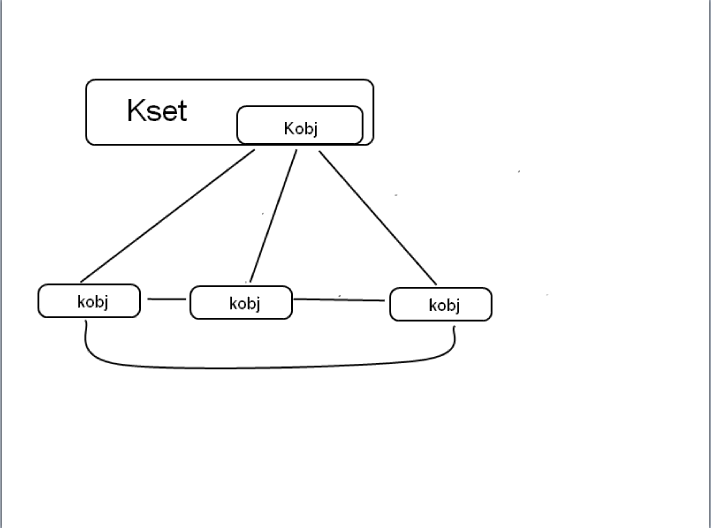
\includegraphics[keepaspectratio,width=0.36\paperwidth]{Pictures/kobject.png}
    \caption{kobject}
    \label{fig:kobject}
  \end{center}
\end{figure}

Nginx 1.0.14 约10万行代码(wc -l返回12万行)。Linux内核2.6.11版本约600万行。SGI STL约有2.4万行。


任何大型的代码都有预分配内存的思想。
Linux上有内存池,slab分配器。
Nginx有slab分配器和内存池。
SGI STL有两级内存分配器,参\ref{sec:memallocidioms}。

封装:struct中只有成员变量的封装,函数指针实际上也是作为变量进行封装。
成员函数封装,在C语言中相当于将操作同一结构的接口放在相同的接口文件中。

继承:ngx\_module\_t中的ctx字段,这种结构实现了继承,ngx\_module\_t相当于基类,而ctx指向派生类成员(包含在ngx\_http\_module\_t等结构中),虽然存储方式不同于C++的派生类。

多态:内核中多态的典型例子是虚拟文件系统。VFS可看做抽象基类,提供struct file\_operations相当于虚函数表。

重载(编译期多态):C语言中经常使用flag变量作为函数参数实现类似重载的效果。

组合:Linux内核中,kobject包含于kset,如图 \ref{fig:kobject}所示。
Linux和中定义有struct list\_head和struct rb\_node(类似于Nginx中的ngx\_queue\_t和ngx\_rbtree\_node\_t),用于生成双链表或红黑树,其他结构中包含它们可以看做组合。


复合型数据结构:如epoll中的epitem节点既属于红黑树,又属于双链表(因为包含list\_head)。前者用于被监控对象插入删除操作(epoll\_ctl),后者是为准备提交给用户的事件。
struct sched\_entity也同时包含struct rb\_node和list\_head。sched\_entity用于CFS(完全公平调度),task\_struct包含了一个sched\_entity。

特性萃取:trait模板、category类体系、重载函数体系。

Nginx用event对象的instance位来处理过期事件问题,instance是bool值,这样做有一定的概率还是会出错,应该改为一个较长的整形,每次
新分配连接时增一,这样,出错的概率极小。

Nginx的过滤模块链表并非链表,而是由各个模块的实现文件中的两个静态变量top和next实现的。




\section{开源代码阅读推荐}
\begin{description}
\item [LwIP] 轻量级协议栈,代码干净,注释详细
\item [memcached] 一套分布式的高速缓存系统, 用CRC-32计算键值后,将数据分散在不同的机器上,数据会以LRU机制替换掉
\item [Redis] Key-Value数据库,C编写,很短,可以全部看下。
\item [Lua] 一门动态语言,提供了一个虚拟机。几万行C代码,简洁优美
\item [uC/OS II]作为一个 RTOS 代码非常不多,分层也挺清楚的
\item [libevent] Libevent是一个轻量级的开源高性能网络库,使用者众多,c语言编写
\item [VxWorks] 美国WindRiver公司RTOS,VxWorks相对简单,模块清晰,代码风格良好
\item [Lucene] 搜索领域的经典项目,是一个高效的,是一个高效的 , 基于Java的全文检索库
\item [Sqlite] sqlite 是一款轻量级的、基于文件的嵌入式数据库,C编写
\item [Duplicity] Python项目。整合已有工具链,实现数据加密增量备份这一任务
\item [Quake III]雷神之锤,一个游戏
\item [trac] 基于Python的软件项目管理系统,拥有强大的bug管理 功能,并集成了Wiki 用于文档管理。它还支持代码管理工具Subversion ,这样可以在 bug管理和Wiki中方便地参考程序源代码
\item [其他] python,LVS,android SDK,BOOST,jdk,spring,openstack,MySQL
\end{description}


















%!Mode:: "TeX:UTF-8"
\section{软件测试}

\subsection{白盒测试}
\textbf{白盒测试(white-box testing)}也称\textbf{结构测试、逻辑驱动测试或基于程序本身的测试}。测试应用程序的内部结构或运作,而不是测试应用程序的功能(即黑盒测试)。在白盒测试时,以编程语言的角度来设计测试案例。测试者输入数据验证数据流在程序中的流动路径,并确定适当的输出,类似测试电路中的节点。测试者了解待测试程序的内部结构、算法等信息,这是从程序设计者的角度对程序进行的测试。

缺点:过分复杂,有时候不切实际,\textbf{它可能会忽视检测规格说明中未被实现的部分}。

主要有基本路径测试(Prime path testing)和逻辑覆盖两种技术设计测试用例。

\textbf{基本路径测试法}是在程序控制流图的基础上,通过分析控制构造的环路复杂性,导出基本可执行路径集合,从而设计测试用例的方法。设计出的测试用例要保证在测试中程序的每个可执行语句至少执行一次。

逻辑覆盖是以程序内部的逻辑结构为基础的设计测试用例的技术。
根据覆盖目标的不同和覆盖源程序语句的详尽程度,逻辑覆盖又可分为:语句覆盖、判定覆盖、条件覆盖、条件/判定覆盖、条件组合覆盖、点覆盖、边覆盖、路径覆盖等。


\subsection{黑盒测试}

\textbf{黑盒测试},软件测试的主要方法之一,也可以称为\textbf{功能测试、数据驱动测试或基于规格说明的测试}。测试者不了解程序的内部情况,不需具备应用程序的代码、内部结构和编程语言的专门知识。只知道程序的输入、输出和系统的功能,这是从用户的角度针对软件界面、功能及外部结构进行测试,而不考虑程序内部逻辑结构。测试案例是依应用系统应该做的功能,照规范、规格或要求等设计。测试者选择有效输入和无效输入来验证是否正确的输出。
此测试方法可适合大部分的软件测试,例如单元测试(unit testing)、集成测试(integration testing)以及系统测试(system testing)。

可采用等价类划分、边界值分析、错误推测法等技术设计测试用例。

等价类划分法是一种典型的、重要的黑盒测试方法,它将程序所有可能的输入数据(有效的和无效的)划分成若干个等价类。然后从每个部分中选取具有代表性的数据当做测试用例进行合理的分类,测试用例由有效等价类和无效等价类的代表组成,从而保证测试用例具有完整性和代表性。

使用边界值分析方法设计测试用例时一般与等价类划分结合起来。但它不是从一个等价类中任选一个例子作为代表,而是将测试边界情况作为重点目标,选取正好等于、刚刚大于或刚刚小于边界值的测试数据。

在测试程序时,人们可能根据经验或直觉推测程序中可能存在的各种错误,从而有针对性地编写检查这些错误的测试用例,这就是错误推测法。



%!Mode:: "TeX:UTF-8"

\section{UML类图}
UML的类图关系分为: 关联、聚合/组合、依赖、泛化(继承)。而其中关联又分为双向关联、单向关联、自身关联。

关系所表现的强弱程度依次为:组合>聚合>关联>依赖。

\subsection{关联}


双向关联:
C1-C2:指双方都知道对方的存在,都可以调用对方的公共属性和方法。

在GOF的设计模式书上是这样描述的:虽然在分析阶段这种关系是适用的,但我们觉得它对于描述设计模式内的类关系来说显得太抽象了,因为在设计阶段关联关系必须被映射为对象引用或指针。对象引用本身就是有向的,更适合表达我们所讨论的那种关系。所以这种关系在设计的时候比较少用到,关联一般都是有向的。

双向关联在代码的表现为双方都拥有对方的一个指针,当然也可以是引用或者是值。

% \begin{figure}[ht]
  % \begin{center}
    % 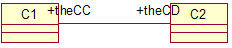
\includegraphics[keepaspectratio,width=0.36\paperwidth]{Pictures/UML/UMLdoubleAssoc.JPG}
    % \caption{双向关联}
    % \label{fig:doubleAssoc}
  % \end{center}
% \end{figure}

% 单向关联:
% C3->C4:表示相识关系,指C3知道C4,C3可以调用C4的公共属性和方法。没有生命期的依赖。一般是表示为一种引用。

% \begin{figure}[ht]
  % \begin{center}
    % 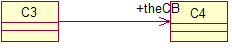
\includegraphics[keepaspectratio,width=0.36\paperwidth]{Pictures/UML/UMLuniAssoc.JPG}
    % \caption{单向关联}
    % \label{fig:uniAssoc}
  % \end{center}
% \end{figure}

% \subsection{组合/聚合}
% 当类之间有整体-部分关系的时候,我们就可以使用组合或者聚合。二者在代码上未必有区别,区别存在于语义上。

% 聚合:表示C9聚合C10,但是C10可以离开C9而独立存在。

% \begin{figure}[ht]
  % \begin{center}
    % 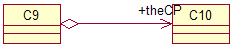
\includegraphics[keepaspectratio,width=0.36\paperwidth]{Pictures/UML/UMLAggregation.JPG}
    % \caption{聚合}
    % \label{fig:Aggregation}
  % \end{center}
% \end{figure}


% \begin{figure}[ht]
  % \begin{center}
    % 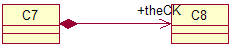
\includegraphics[keepaspectratio,width=0.36\paperwidth]{Pictures/UML/UMLComposition.JPG}
    % 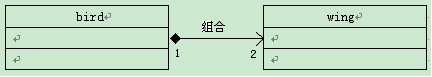
\includegraphics[keepaspectratio,width=0.36\paperwidth]{Pictures/UML/UmlCompositionNumbered.png}
    % \caption{组合}
    % \label{fig:UMLComposition}
  % \end{center}
% \end{figure}
% 组合(也有人称为包容、合成):一般是实心菱形加实线箭头表示,如上图所示,表示的是C8被C7包容,而且C8不能离开C7而独立存在。但这是视问题域而定的,例如在关心汽车的领域里,轮胎是一定要组合在汽车类中的,因为它离开了汽车就没有意义了。但是在卖轮胎的店铺业务里,就算轮胎离开了汽车,它也是有意义的,这就可以用聚合了。在《敏捷开发》中还说到,A组合B,则A需要知道B的生存周期,即可能A负责生成或者释放B,或者A通过某种途径知道B的生成和释放。



% 合成(Composition)是一种强的“拥有”关系,体现了严格的部分和整体的关系,部分和整体的生命周期一样。
% 合成关系用实心菱形加实线箭头表示。数字1、2是基数,表明这一端的类可以有几个实例。n表示可能有无数个实例。关联和聚合也可以有基数。

% \subsection{依赖}

% 指C5可能要用到C6的一些方法,也可以这样说,要完成C5里的所有功能,一定要有C6的方法协助才行。C5依赖于C6的定义,一般是在C5类的头文件中包含了C6的头文件。注意,要避免双向依赖。一般来说,不应该存在双向依赖。

% 在形式上一般是A中的某个方法把B的对象作为参数使用(假设A依赖于B)。如下:
% \begin{verbatim}
% #include "B.h"
% class A
% ...{
          % void Func(B &b);
% }
% \end{verbatim}


% \begin{figure}[ht]
  % \begin{center}
    % 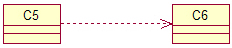
\includegraphics[keepaspectratio,width=0.36\paperwidth]{Pictures/UML/UMLDependancy.JPG}
    % \caption{依赖}
    % \label{fig:UMLDependancy}
  % \end{center}
% \end{figure}

% 那依赖和聚合/组合、关联等有什么不同呢?

% 关联是类之间的一种关系,例如老师教学生,老公和老婆,水壶装水等就是一种关系。这种关系是非常明显的,在问题领域中通过分析直接就能得出。

% 依赖是一种弱关联,只要一个类用到另一个类,但是和另一个类的关系不是太明显的时候(可以说是“uses”了那个类),就可以把这种关系看成是依赖,依赖也可说是一种偶然的关系,而不是必然的关系,就是“我在某个方法中偶然用到了它,但在现实中我和它并没多大关系”。例如我和锤子,我和锤子本来是没关系的,但在有一次要钉钉子的时候,我用到了它,这就是一种依赖,依赖锤子完成钉钉子这件事情。
% 组合是一种整体-部分的关系,在问题域中这种关系很明显,直接分析就可以得出的。例如轮胎是车的一部分,树叶是树的一部分,手脚是身体的一部分这种的关系,非常明显的整体-部分关系。

% 上述的几种关系(关联、聚合/组合、依赖)在代码中可能以指针、引用、值等的方式在另一个类中出现,不拘于形式,但在逻辑上他们就有以上的区别。

% 这里还要说明一下,所谓的这些关系只是在某个问题域才有效,离开了这个问题域,可能这些关系就不成立了,例如可能在某个问题域中,我是一个木匠,需要拿着锤子去干活,可能整个问题的描述就是我拿着锤子怎么钉桌子,钉椅子,钉柜子;既然整个问题就是描述这个,我和锤子就不仅是偶然的依赖关系了,我和锤子的关系变得非常的紧密,可能就上升为组合关系(让我突然想起武侠小说的剑不离身,剑亡人亡...)。这个例子可能有点荒谬,但也是为了说明一个道理,就是关系和类一样,它们都是在一个问题领域中才成立的,离开了这个问题域,他们可能就不复存在了。


% \subsection{泛化}
% 泛化(Generalization)表示一个更泛化的元素和一个更具体的元素之间的关系。泛化是用于对继承进行建模的UML元素。在Java中,用extends关键字来直接表示这种关系。

% \begin{figure}[ht]
  % \begin{center}
    % 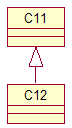
\includegraphics[keepaspectratio,width=0.05\paperwidth]{Pictures/UML/UMLinheri.JPG}
    % \caption{泛化(OOP中“继承”同泛化方向相反)}
    % \label{fig:UMLinheri}
  % \end{center}
% \end{figure}

% \subsection{实现(Realization)}
% OOP中的接口继承用实现(Realization)关系进行建模。
% 实现关系指定两个实体之间的一个合同。换言之,一个实体定义一个合同,而另一个实体保证履行该合同。
% 对Java应用程序进行建模时,实现关系可直接用implements关键字来表示。

% \begin{figure}[ht]
% \centering
	% \begin{minipage}[t]{0.4\textwidth}  
	 % 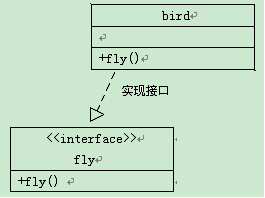
\includegraphics[keepaspectratio,width=0.2\paperwidth]{Pictures/UML/UmlInterfaceRec.png}
    % \caption{接口继承矩形表示法}
    % \label{fig:UMLInterfaceInheri}
	% \end{minipage}
	% \begin{minipage}[t]{0.4\textwidth} 
   % 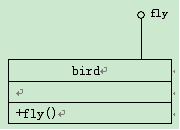
\includegraphics[keepaspectratio,width=0.2\paperwidth]{Pictures/UML/UmlInterfaceCandy.png}
    % \caption{接口继承棒棒糖表示法}
    % \label{fig:UMLInterfaceInheri}
	% \end{minipage} 
% \end{figure}



\clearpage








\end{document}
